\documentclass[12pt,a4paper]{article}
\usepackage{graphicx}
\usepackage{amsmath}
\usepackage{float}
\usepackage{ amssymb }
\usepackage{siunitx}
\usepackage[utf8]{inputenc}
\usepackage[czech]{babel}

\begin{document}

%----------------------------------------------------------------------------------------
%	TITLE PAGE
%----------------------------------------------------------------------------------------
\begin{titlepage}
	\centering
	{\scshape\Large Vysoké učení technické v Brně \par}
	\vspace{0.5cm}
	{\scshape Fakulta informačních technologii \par}
	\vspace{1.5cm}
	{\huge\bfseries IEL - Projekt\par}
	\vspace{2cm}
	{\Large\itshape Jozef Hruška\par}
	\vfill

	{\large \today\par}
\end{titlepage}

%----------------------------------------------------------------------------------------
%	1ST ASSIGNMENT
%----------------------------------------------------------------------------------------
\section{Skupina - H}
\begin{tabular}{ l l l l l }
  U\textsubscript{1} = 135V & U\textsubscript{2} = 80V & R\textsubscript{1} = 680 \si{\ohm} & R\textsubscript{2} = 600 \si{\ohm} & R\textsubscript{3} = 260 \si{\ohm} \\
  R\textsubscript{4} = 310 \si{\ohm} & R\textsubscript{5} = 575 \si{\ohm} & R\textsubscript{6} = 870 \si{\ohm} & R\textsubscript{7} = 355 \si{\ohm} & R\textsubscript{8} = 265 \si{\ohm} \\
\end{tabular}

\begin{figure}[h]
\centering
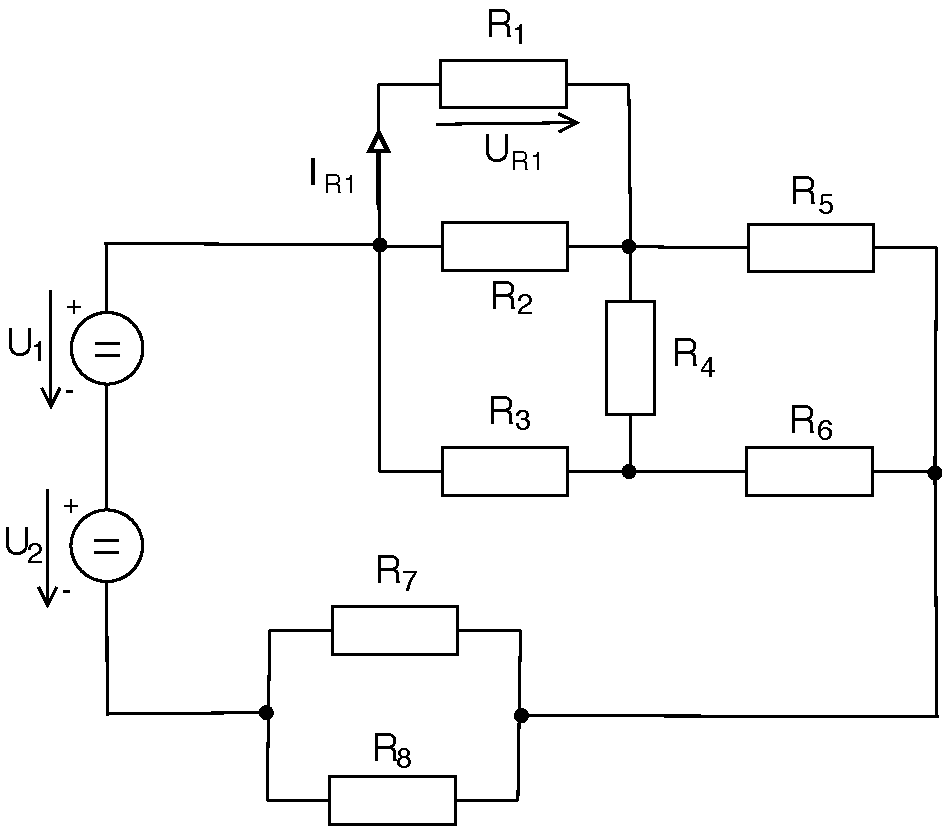
\includegraphics[width=0.5\textwidth]{Circuits/1-A.pdf}
\caption{Východzí obvod projektu.}
\end{figure}

\begin{minipage}{.33\linewidth}
\begin{align*}
        R_{78} &= \frac{R_7 * R_8}{R_7 + R_8} \\[0.5ex]
	R_{78} &= \frac{355 * 265}{355 + 265} \\[0.5ex]
	R_{78} &= \frac{18815}{124} \si{\ohm} \\[0.5ex]
\end{align*}
\end{minipage}%
\begin{minipage}{.33\linewidth}
\begin{align*}
        R_{12} &= \frac{R_1 * R_2}{R_1 + R_2} \\[0.5ex]
	R_{12} &= \frac{680 * 600}{680 + 600} \\[0.5ex]
	R_{12} &= \frac{1275}{4} \si{\ohm} \\[0.5ex]
\end{align*}
\end{minipage}%
\begin{minipage}{.33\linewidth}
\begin{align*}
        U_{12} &= U_1 + U_2 \\[0.5ex]
	U_{12} &= 135 + 80 \\[0.5ex]
	U_{12} &= 215V \\[0.5ex]
\end{align*}
\end{minipage}

\begin{figure}[h]
\centering
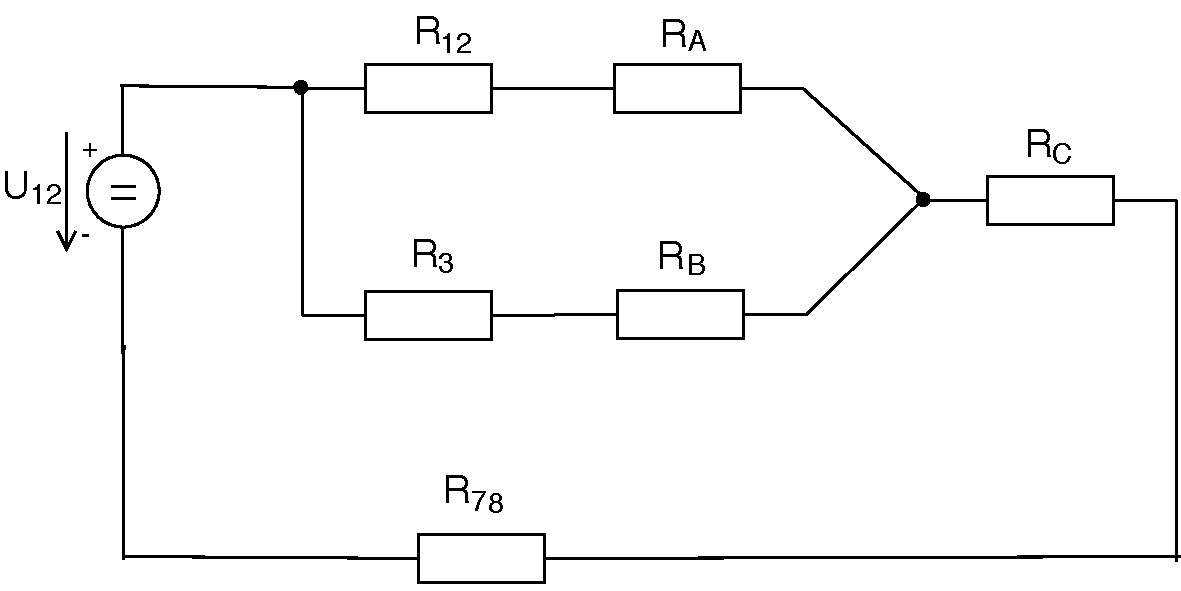
\includegraphics[width=0.5\textwidth]{Circuits/1-B.pdf}
\caption{Evivalentný obvod.}
\end{figure}

\begin{minipage}{.33\linewidth}
\begin{align*}
        R_{A} &= \frac{R_4 * R_5}{R_4 + R_5} \\[0.5ex]
	R_{A} &= \frac{310 * 575}{310 + 575} \\[0.5ex]
	R_{A} &= 101,567 \si{\ohm} \\[0.5ex]
\end{align*}
\end{minipage}%
\begin{minipage}{.33\linewidth}
\begin{align*}
        R_{B} &= \frac{R_4 * R_6}{R_4 + R_6} \\[0.5ex]
	R_{B} &= \frac{310 * 870}{310 + 870} \\[0.5ex]
	R_{B} &= \frac{17980}{117} \si{\ohm} \\[0.5ex]
\end{align*}
\end{minipage}%
\begin{minipage}{.33\linewidth}
\begin{align*}
        R_{C} &= \frac{R_5 * R_6}{R_5 + R_6} \\[0.5ex]
	R_{C} &= \frac{575 * 870}{575 + 870} \\[0.5ex]
	R_{C} &= \frac{33350}{117} \si{\ohm} \\[0.5ex]
\end{align*}
\end{minipage}

\begin{minipage}{.33\linewidth}
\begin{align*}
        R_{C78} &= R_C + R_{78} \\[0.5ex]
	R_{C78} &= \frac{33350}{117} + \frac{18815}{124} \\[0.5ex]
	R_{C78} &= 436,7766 \si{\ohm} \\[0.5ex]
\end{align*}
\end{minipage}%
\begin{minipage}{.33\linewidth}
\begin{align*}
        R_{A12} &= R_A + R_{12} \\[0.5ex]
	R_{A12} &= 101,567 + \frac{1275}{4} \\[0.5ex]
	R_{A12} &= 420,317 \si{\ohm} \\[0.5ex]
\end{align*}
\end{minipage}%
\begin{minipage}{.33\linewidth}
\begin{align*}
        R_{B3} &= R_B + R_3 \\[0.5ex]
	R_{B3} &= \frac{17980}{117} + 260 \\[0.5ex]
	R_{B3} &= \frac{48400}{117} \si{\ohm} \\[0.5ex]
\end{align*}
\end{minipage}

\begin{minipage}{.5\linewidth}
\begin{align*}
        R_{AB123} &= \frac{R_{A12} * R_{B3}}{R_{A12} + R_{B3}} \\[0.5ex]
	R_{AB123} &= \frac{420,317 * \frac{48400}{117}}{420,317 + \frac{48400}{117}} \\[0.5ex]
	R_{AB123} &= 208,4848 \si{\ohm} \\[0.5ex]
\end{align*}
\end{minipage}%
\begin{minipage}{.5\linewidth}
\begin{align*}
        R_{EKV} &= R_{AB123} + R_{C78} \\[0.5ex]
	R_{EKV} &= 208,4848 + 436,7766 \\[0.5ex]
	R_{EKV} &= 645,2614 \si{\ohm} \\[0.5ex]
\end{align*}
\end{minipage}

\begin{minipage}{.33\linewidth}
\begin{align*}
       	I &= \frac{U_{12}}{R_{EKV}} \\[0.5ex]
	I &= \frac{215}{645,2614}\\[0.5ex]
	I &= 0,3332 A \\[0.5ex]
\end{align*}
\end{minipage}%
\begin{minipage}{.33\linewidth}
\begin{align*}
        U_{RAB123} &= R_{AB123} * I \\[0.5ex]
	U_{RAB123} &= 208,4848 * 0,3332 \\[0.5ex]
	U_{RAB123} &= 69,4671 V = U_{RA12}\\[0.5ex]
\end{align*}
\end{minipage}%
\begin{minipage}{.33\linewidth}
\begin{align*}
        I_{A12} &= \frac{U_{RA12}}{R_{A12}} \\[0.5ex]
	I_{A12} &= \frac{69,4671}{420,317} \\[0.5ex]
	I_{A12} &= 0,1653 \\[0.5ex]
\end{align*}
\end{minipage}

\begin{equation}
	U_{R12} = R_{12} * I_{A12} = 52,6894 V = U_{R1} \\
\end{equation}

\begin{equation}
	I_{R1} = \frac{U_{R1}}{R_1} = \frac{52,6894}{680} = 0,0775 A 
\end{equation}
%----------------------------------------------------------------------------------------
%	2ND ASSIGNMENT
%----------------------------------------------------------------------------------------
\newpage
\section{Skupina - A}
\begin{tabular}{ l l l }
  U\textsubscript{1} = 50V & U\textsubscript{2} = 100V & R\textsubscript{1} = 525 \si{\ohm} \\
  R\textsubscript{2} = 620 \si{\ohm} & R\textsubscript{3} = 210 \si{\ohm} & R\textsubscript{4} = 530 \si{\ohm} \\
\end{tabular}

 \begin{minipage}{\linewidth}
      \centering
      \begin{minipage}{0.45\linewidth}
          \begin{figure}[H]
              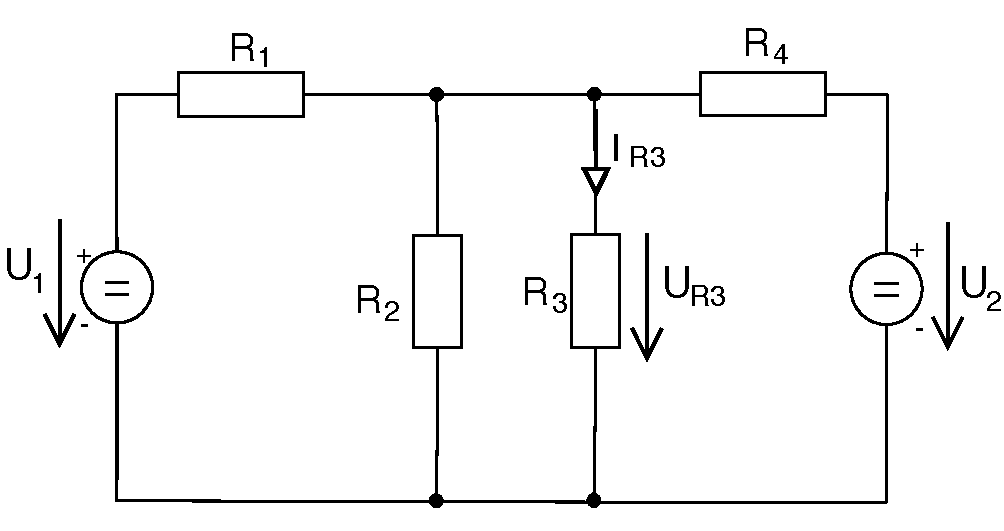
\includegraphics[width=\linewidth]{Circuits/2-A.pdf}
          \end{figure}
      \end{minipage}
      \hspace{0.05\linewidth}
      \begin{minipage}{0.45\linewidth}
      	\begin{align*}
        		R_{23} &= \frac{R_2 * R_3}{R_2 + R_3} = \frac{620 * 210}{620 + 210} \\[0.5ex]
			R_{23} &= \frac{13020}{83} \si{\ohm} \\[0.5ex]
		\end{align*}
      \end{minipage}
  \end{minipage}
  
  \begin{minipage}{\linewidth}
      \centering
      \begin{minipage}{0.45\linewidth}
          \begin{figure}[H]
              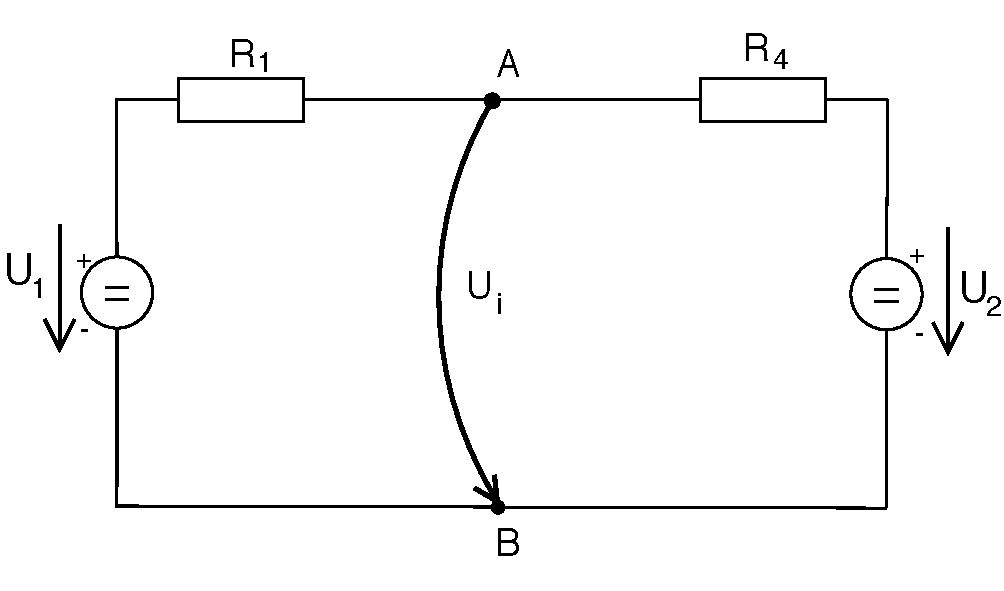
\includegraphics[width=\linewidth]{Circuits/2-B.pdf}
          \end{figure}
      \end{minipage}
      \hspace{0.05\linewidth}
      \begin{minipage}{0.45\linewidth}
      	\begin{align*}
        		U_1 + U_{R1} + U_{R4} - U_2 &= 0 \\[0.5ex]
        		U_1 + R_1I_X + R_4I_X - U_2 &= 0 \\[0.5ex]
        		50 + 525I_X + 530I_X - 100 &= 0 \\[0.5ex]
        		1055I_X &= 50 \\[0.5ex]
        		I_X &= \frac{10}{211}  \\[0.5ex]
		\end{align*}
      \end{minipage}
  \end{minipage}
  
  \begin{minipage}{\linewidth}
      \centering
      \begin{minipage}{0.45\linewidth}
          \begin{figure}[H]
              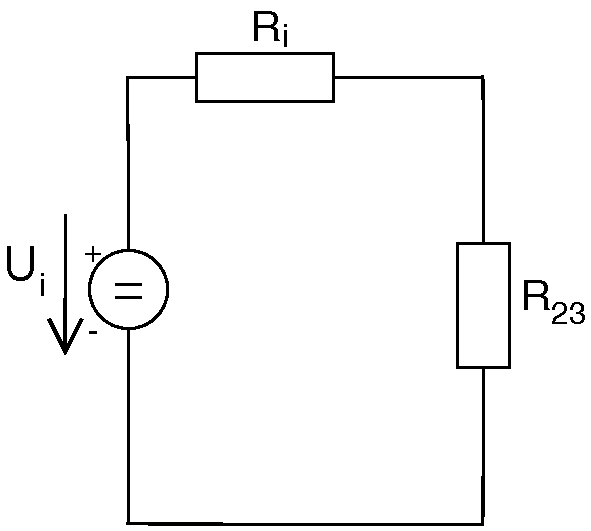
\includegraphics[width=\linewidth]{Circuits/2-C.pdf}
          \end{figure}
      \end{minipage}
      \hspace{0.05\linewidth}
      \begin{minipage}{0.45\linewidth}
      	\begin{align*}
        		R_4I_X + U_i - U_2 &= 0 \\[0.5ex]
        		(530 * \frac{10}{211}) + U_i - 100 &= 0 \\[0.5ex]
        		U_i = 100 - \frac{5300}{211} &= \frac{15800}{211} \\[5mm]
        		R_i = \frac{R_1*R_4}{R_1+R_4} &= \frac{525 * 530}{525 + 530} \\[0.5ex]
        		R_i &= 263,7441 \si{\ohm} \\[0.5ex]
		\end{align*}
      \end{minipage}
  \end{minipage}
  
  \begin{align*}
  	I_{R23} &= \frac{U_i}{R_i + R_{23}} \\[0.5ex]
  	I_{R23} &= \frac{\frac{15800}{211}}{263,7441 + \frac{13020}{83}} \\[0.5ex]
  	I_{R23} &= 0,178 A
  \end{align*}
  
    \begin{align*}
  	U_{R23} &= R_{23} * I_{R23} \\[0.5ex]
  	U_{R23} &= \frac{13020}{83} * 0,178 \\[0.5ex]
  	U_{R23} &= 27,9224 V = U_{R3}
  \end{align*}
  
      \begin{align*}
  	I_{R3} &= \frac{U_{R23}}{R_3} \\[0.5ex]
  	I_{R3} &= \frac{27,9224}{210} \\[0.5ex]
  	I_{R3} &= 132,96 mA
  \end{align*}
  
%----------------------------------------------------------------------------------------
%	3RD ASSIGNMENT
%----------------------------------------------------------------------------------------
\newpage
\section{Skupina - C}
\begin{tabular}{ l l l l }
  U = 110V & I\textsubscript{1} = 0.85A & I\textsubscript{2} = 0.75A & R\textsubscript{1} = 44 \si{\ohm}   \\
  R\textsubscript{2} = 31 \si{\ohm} & R\textsubscript{3} = 56 \si{\ohm} & R\textsubscript{4} = 20 \si{\ohm} & R\textsubscript{5} = 30 \si{\ohm} \\
\end{tabular}

  \begin{minipage}{\linewidth}
      \centering
      \begin{minipage}{0.45\linewidth}
          \begin{figure}[H]
              \includegraphics[width=\linewidth]{Circuits/3-A.pdf}
          \end{figure}
      \end{minipage}
      \hspace{0.05\linewidth}
      \begin{minipage}{0.45\linewidth}
          \begin{figure}[H]
              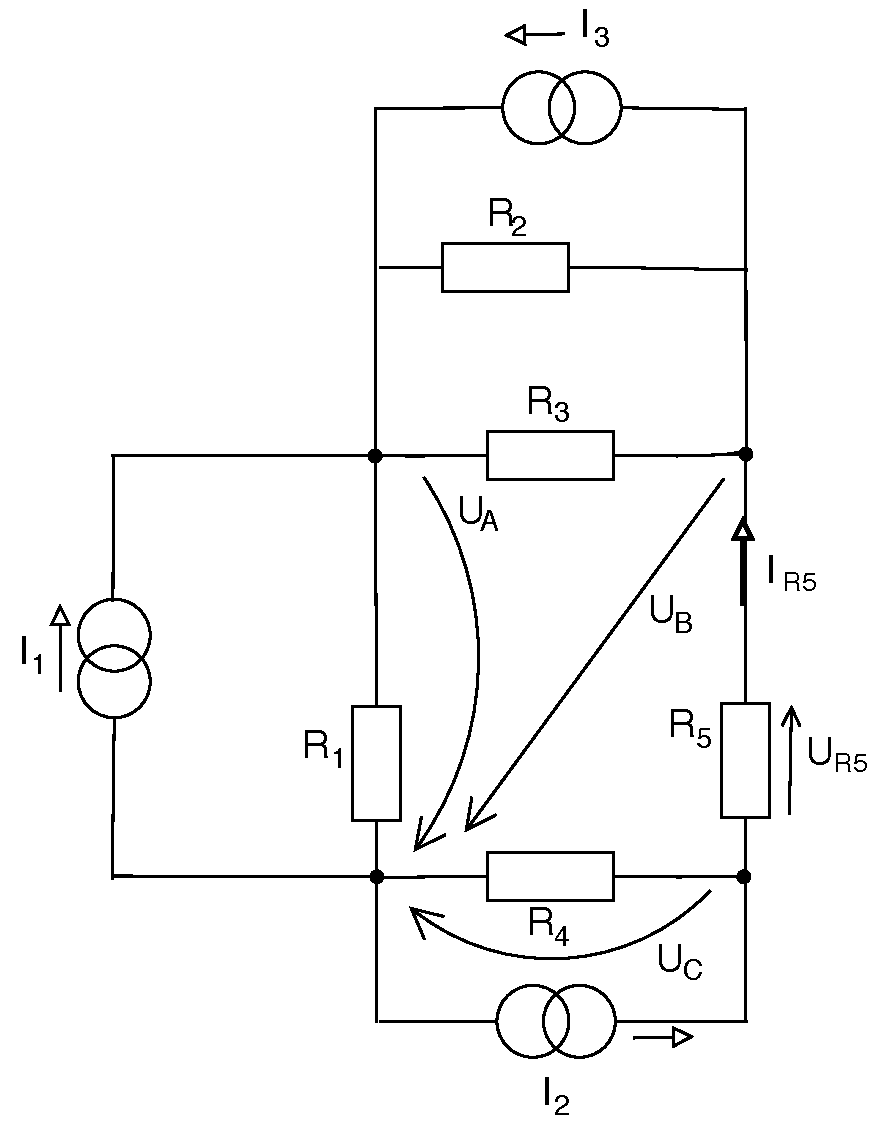
\includegraphics[width=\linewidth]{Circuits/3-B.pdf}
          \end{figure}
      \end{minipage}
  \end{minipage}
  
  \begin{tabular}{ l l l }
  	$I_3 = \frac{U}{R2} = \frac{110}{31}$ & $G_1 = \frac{1}{R_1} = \frac{1}{44}$ & $G_2 = \frac{1}{R_2} = \frac{1}{31}$ \\
  	 $G_3 = \frac{1}{R_3} = \frac{1}{56}$ & $G_4 = \frac{1}{R_4} = \frac{1}{20}$ & $G_5 = \frac{1}{R_5} = \frac{1}{30}$ \\
  \end{tabular}
  
  \vspace{1cm}
  
\[
\begin{bmatrix}
    G_1 + G_2 + G_3       & -G_2 - G_3 & 0 \\
    -G_2 - G_3       & G_2 + G_3 + G_5 & -G_5  \\
    0      & -G_5 & G_4 + G_5
\end{bmatrix}
=
\begin{bmatrix}
    I_1 + I_3 \\
    -I_3 \\
    I_2 \\
\end{bmatrix}
\]

 \vspace{0.3cm}
 Nahradíme si postupne stĺpce v hlavnej matici a vypočítame determinanty.
  \vspace{0.3cm}

  \begin{tabular}{ l l l l l }
  	$\Delta = \frac{4957}{22915200}$ & $\Delta_B = \frac{-257713}{190960000}$ & $\Delta_C = \frac{32243}{22915200}$ & $U_B = \frac{\Delta_B}{\Delta}$ & $U_C = \frac{\Delta_C}{\Delta}$ \\
  \end{tabular}
  
  \vspace{0.5cm}
  
    \begin{minipage}{\linewidth}
      \centering
      \begin{minipage}{0.45\linewidth}
           	\begin{align*}
       			-U_{R5} &= U_B - U_C \\
       			-U_{R5} &= -6,2388 - 6,5045  \\
       			-U_{R5} &= -12,7433 V 
		\end{align*}
      \end{minipage}
      \hspace{0.05\linewidth}
      \begin{minipage}{0.45\linewidth}
           	\begin{align*}
       			I_{R5} &= \frac{U_{R5}}{R_5} = \frac{12,7433}{30}  \\
       			I_{R5} &= 0,4248 A  \\
		\end{align*}
      \end{minipage}
  \end{minipage}
  
%----------------------------------------------------------------------------------------
%	4TH ASSIGNMENT
%----------------------------------------------------------------------------------------
\newpage
\section{Skupina - H}
  
%----------------------------------------------------------------------------------------
%	5TH ASSIGNMENT
%----------------------------------------------------------------------------------------
\newpage
\section{Skupina - A}
\begin{tabular}{ l l l l }
  U = 20V & C = 50F & R = 10\si{\ohm} & $\mathcal{U}_C(0) = 9V$  \\
\end{tabular}

\begin{minipage}{\linewidth}
      \centering
      \begin{minipage}{0.45\linewidth}
          \begin{figure}[H]
              \includegraphics[width=\linewidth]{Circuits/5-A.pdf}
          \end{figure}
      \end{minipage}
      \hspace{0.05\linewidth}
      \begin{minipage}{0.45\linewidth}
          	\begin{align*}
       			I = \frac{U_{R5}}{R_5}  \\[5mm]
       			U_R + U_C - U = 0  \\
       			U_R = U - U_C  \\[5mm]
       			U_C' = \frac{I}{C} = \frac{U_R}{RC} = \frac{U - U_C}{RC}  \\[5mm]
       			U_C' + \frac{U_C}{RC} = \frac{U}{RC}
		\end{align*}
      \end{minipage}
  \end{minipage}
  
  \vspace{1cm}
  
  \begin{minipage}{\linewidth}
      \centering
      \begin{minipage}{0.45\linewidth}
          	\begin{align*}
       			\lambda + \frac{1}{RC} = 0  \\
       			\lambda = \frac{-1}{RC}  \\[5mm]
       			\mathcal{U}_C(t) = K(t)e^{\lambda t} \\
       			\mathcal{U}_C(t) = K(t)e^{\frac{t}{RC}}
		\end{align*}
      \end{minipage}
      \hspace{0.05\linewidth}
      \begin{minipage}{0.45\linewidth}
      	       	\begin{align*}
       			 \mathcal{U}_C'= K'(t)(\frac{-1}{RC})e^{\frac{-t}{RC}} + K(t)(\frac{-1}{RC})e^{\frac{-t}{RC}}  \\[5mm]
       			 K'(t)e^{\frac{-t}{RC}} + K(t)(\frac{-1}{RC})e^{\frac{-t}{RC}} + K(t)(\frac{1}{RC})e^{\frac{-t}{RC}} = \frac{U}{RC} \\
       			 K'(t)e^{\frac{-t}{RC}} = \frac{U}{RC} \\
       			 K'(t) = \frac{U}{RC}e^{\frac{-t}{RC}}
		\end{align*}
      \end{minipage}
  \end{minipage}
  
\newpage

\begin{center}
 \begin{tabular}{|c |c |c|} 
 \hline
 Úloha & Skupina & Výsledky\\ [0.5ex] 
 \hline\hline
 1 & H & $U_{R1} = 52,6894V, I_{R1} = 77,5mA $  \\ 
 \hline
 2 & A & $U_{R3} = 27,9224V, I_{R3} = 132,96mA$  \\
 \hline
 3 & C & $U_{R5} = 12,7433V, I{R5} = 424,8mA $ \\
 \hline
 4 & H & \\
 \hline
 5 & A & \\ [1ex] 
 \hline
\end{tabular}
\end{center}

\end{document}